\documentclass[border=3pt]{standalone}
\usepackage{amsmath,amssymb} 
\usepackage{mathtools}

\makeatletter
\def\mathcolor#1#{\@mathcolor{#1}}
\def\@mathcolor#1#2#3{%
  \protect\leavevmode
  \begingroup
    \color#1{#2}#3%
  \endgroup
}         
\makeatother


\usepackage[OT1]{fontenc}
\renewcommand*\familydefault{\sfdefault}
\usepackage{xcolor}
\usepackage{physics}
\usepackage{siunitx}

\usepackage{ifthen}
\usepackage{tikz}
\usetikzlibrary[
    arrows,
    arrows.meta,
    positioning,
    backgrounds,
    calc,
    shadings,
    decorations,
    decorations.pathmorphing,
    decorations.markings,
    patterns,
]

\usepackage{pgfplots}
% \usepgfplotslibrary{fillbetween}

\usepackage{ctex}
%%%%%%%%%%%%%%%%%%%%%%%%%%%%%%%%%%%%%%%%%%%%%%%%%%%%%%%%%%%%%%%%%%%%%%%%%%%%%%%%
\begin{document}
%%%%%%%%%%%%%%%%%%%%%%%%%%%%%%%%%%%%%%%%%%%%%%%%%%%%%%%%%%%%%%%%%%%%%%%%%%%%%%%%
\begin{tikzpicture}
  [x=1in, y=1in]
  \node (pub_year) [anchor=north east, text width=4in, inner sep=0pt] at (-1.0, 0) {
    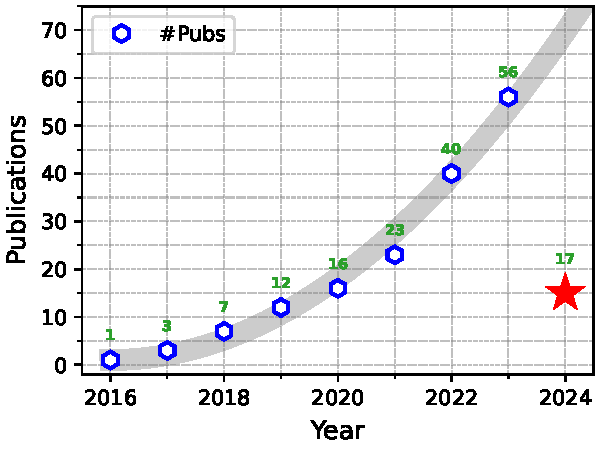
\includegraphics[width=1.0\linewidth]{pub_per_year.pdf}
  };
  \node (pub_pie) [below=20pt of pub_year, text width=5in, inner sep=0pt] {
    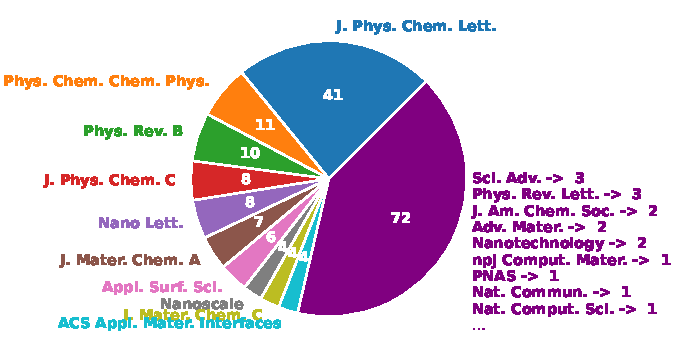
\includegraphics[width=1.0\linewidth]{pub_pie.pdf}
  };


  \shade[ball color=blue] (0, 0)  circle (3pt);

  \node[text width=1.5in, align=right, font=\Large, blue] at (0, 0) {姓名};
  \node[text width=2.0in, align=left, font=\Large, black] at (2, 0) {单位};
  \draw[line width=2pt, gray] (-0.75in, -0.25) -- ++(3.5in, 0);

  \foreach  \usr/\affl [count=\ii starting from 1] in {
    Shaul Mukamel\\(美国科学院院士)/美国加州大学尔湾分校,
    ShiXue Dow/澳大利亚伍伦贡大学,
    Saidi A. Wissam/美国匹兹堡大学,
    Noa Marom/美国卡耐基梅隆大学,
    Oleg V. Prezhdo/美国南加州大学,
    K.M. Ho/美国爱荷华州立大学,
    A. Akimov/美国纽约大学布法罗分校,
    Thomas Frauenheim/德国布莱梅大学,
    Aron Walsh/英国伦敦皇家学院,
    杨金龙(中科院院士)/中国科学技术大学,
    龚新高(中科院院士)/复旦大学,
    赵纪军/华南师范大学(原大连理工),
    王金兰/东大大学,
    戴佳钰/国防科技大学,
    张红/四川大学,
    赵明文/山东大学,
    周苗/北京航空航天大学,
    陆瑞锋/南京理工大学,
    曾海波/南京理工大学,
  }{
    \node[text width=1.5in, align=right, blue] at (0, -{\ii*0.28 - 0.3}) {\usr};
    \node[text width=2.0in, align=left, black] at (2, -{\ii*0.28 - 0.3}) {\affl};
  }
\end{tikzpicture}
%%%%%%%%%%%%%%%%%%%%%%%%%%%%%%%%%%%%%%%%%%%%%%%%%%%%%%%%%%%%%%%%%%%%%%%%%%%%%%%%
\end{document}
